\documentclass[12pt,a4paper]{ctexart}

\usepackage{geometry}
\usepackage{graphicx}
\usepackage{array}
\usepackage{booktabs}
\usepackage{amsmath}
\usepackage{amssymb}
\usepackage{xeCJK}
\usepackage{tikz}
\usepackage{titlesec}

% 页面设置
\geometry{
    top=2.5cm,
    bottom=2.5cm,
    left=2.8cm,
    right=2.8cm
}

% 定义 section* 格式
\titleformat{\section}
  {\zihao{-3}\heiti\bfseries}
  {}
  {0em}
  {}
\titlespacing*{\section}{0pt}{0.5cm}{0.3cm}  % 左缩进、上间距、下间距


% 取消页码（封面）
\pagestyle{empty}

% 定义等长下划线命令（固定宽度 6.5cm，左对齐）
\newcommand{\infofill}[1]{{\zihao{4}\songti\underline{\makebox[6.5cm][c]{#1}}}}

% 定义内容区块命令
\newcommand{\reportsection}[2]{%
    \noindent{\zihao{-3}\heiti\bfseries #1（#2分）}
    \vspace{0.3cm}
    
    \noindent\rule{\textwidth}{0.4pt}
    \vspace{6cm}
}

% 设置中文字体
\setCJKmainfont{SimSun}  % 宋体，可根据系统改为 Noto Serif CJK SC 等

\begin{document}
% ==================== 封面页 ====================
\begin{titlepage}
    \centering
    \vspace*{1.5cm}
    % 校徽占位（正方形示例图）
    
\includegraphics[width=5cm,height=5cm]{images/image-2026-09-07-14-57-04.png}
    
    \vspace{1.8cm}
    
    % 中山大学
    {\zihao{1}\heiti\bfseries 中山大学}
    
    \vspace{0.9cm}
    
    % 微电子科学与技术学院
    {\zihao{2}\heiti 微电子科学与技术学院}
    
    \vspace{0.9cm}
    
    % 课程名称
    {\zihao{2}\heiti 《集成电路元器件特性表征实验》}
    
    \vspace{0.9cm}
    
    % 实验报告
    {\zihao{1}\heiti\bfseries 实验报告}
    
    \vspace{3cm}
    
    % 信息表格
    

    % 信息表格（无任何框线，无横线，无竖线）
    \begin{tabular}{@{}>{\zihao{4}\heiti}r @{\hspace{1.2em}} l@{}}
        实验主题      & \infofill{四探针法测量电阻率与方块电阻}        \\[0.8cm]
        姓\quad\quad 名 & \infofill{徐睿琳}   \\[0.8cm]
        学\quad\quad 号 & \infofill{23342107} \\[0.8cm]
        实验日期      & \infofill{\today}   \\[0.8cm]
    \end{tabular}
    
    \vfill
\end{titlepage}

% ==================== 内容页 ====================
\newpage
\pagestyle{plain}
\setcounter{page}{2}

\section*{实验目的（5分）}
\begin{enumerate}
    \item 掌握四探针法测量半导体电阻率的基本原理与普适公式，理解点电流源等势面模型及边界、厚度修正的适用条件。
    \item 掌握薄层电阻（方块电阻）的定义及其与体电阻率的关系，熟悉双电测组合四探针法的测量原理与修正优势。
    \item 掌握四线法接线与源表操作，学会通过变电流测试与多点测试评价电阻率（方阻）的变化率与不均匀度，并了解由电阻率推算掺杂浓度的方法。
\end{enumerate}

\section*{实验原理（10分）}

\subsection*{1. 四探针法基本原理}
在半无穷大均匀样品表面，探针 1、4 通入电流 $I$，探针 2、3 测量电势差 $V_{23}$。由点电流源的半球面等势分布，电势叠加得普遍公式
\begin{equation}
\rho=\frac{2\pi V_{23}}{I}\Big/\left(\frac{1}{r_{12}}-\frac{1}{r_{42}}-\frac{1}{r_{13}}+\frac{1}{r_{43}}\right)
\end{equation}
对等间距 $S$ 的直线型四探针，$r_{12}=r_{34}=S$、$r_{42}=r_{13}=2S$，化简为
\begin{equation}
\rho=\frac{2\pi S V_{23}}{I}
\end{equation}
该式适用于样品厚度及探针至边界距离均大于 $4S$ 的情形。

\subsection*{2. 厚度与边界修正}
当上述条件不满足时引入修正系数 $B_0$：
\begin{equation}
\rho=\frac{2\pi S}{B_0}\frac{V_{23}}{I}
\end{equation}
$B_0$ 由样品厚度、边界距离及几何位置决定。

\subsection*{3. 极薄样品与方块电阻}
当样品厚度 $d\ll S$ 且横向尺寸视为无穷大时，等势面近似为高 $d$ 的圆柱面，有
\begin{equation}
\rho=\frac{\pi}{\ln 2}\,d\,\frac{V_{23}}{I}=4.5324\,d\,\frac{V_{23}}{I}
\end{equation}
定义薄层电阻（方块电阻）
\begin{equation}
R_{sh}=\frac{\rho}{d}=\frac{\pi}{\ln 2}\frac{V_{23}}{I}=4.5324\frac{V_{23}}{I}
\end{equation}

其单位为 $\Omega/\square$，与样品横向尺寸无关，仅取决于材料与厚度。

\subsection*{4. 双电测组合四探针法}
采用 $I_{14}V_{23}$ 与 $I_{13}V_{24}$ 两种组合，并改变电流方向各测一次取平均，由比值 $V_{23}/V_{24}$ 确定修正因子 $K$，则
\begin{equation}
R_{sh}=K\frac{V_{23}}{I}
\end{equation}
该方法结果与探针间距无关，可消除针距不等及机械游移的影响，并自动修正边界效应。

\subsection*{5. 变化率与不均匀度}
变化率表征同一点测量结果随激励电流的漂移程度；不均匀度定义为
\begin{equation}
E=\frac{\Delta \rho}{\bar{\rho}}\times 100\%\approx
\frac{\rho_{\max}-\rho_{\min}}{(\rho_{\max}+\rho_{\min})/2}\times 100\%
\end{equation}
用于评价样品电学参数的面内均匀性。

\section*{实验设备和步骤（5分）}

\subsection*{1. 实验设备}
同惠 TH1992B 源表、四探针台、硅片样品、ITO 透明导电薄膜样品。

\subsection*{2. 实验步骤}
\begin{enumerate}
    \item 按四线法连接探针与源表：1、4 线接 Force，2、3 线接 Sense。
    \item 源表设为电流源模式、四线制感应，电压与电流量程置于自动。
    \item 放置样品，操作探针台下压探针，确认电流正常流经样品。
    \item 硅片测试：固定测点，依次施加 $0.1\sim0.6\ \mathrm{mA}$ 电流，记录正反向 $+V_{23}$、$-V_{23}$，计算电阻率及变化率。
    \item 硅片不均匀度测试：电流固定为 $0.1\ \mathrm{mA}$，在样品五个不同区域测量，计算电阻率不均匀度。
    \item ITO 测试：同法测量方块电阻的变化率与不均匀度。
\end{enumerate}

\section*{实验数据分析（50分）}

\subsection*{1. 数据处理方法}
为消除探针—样品接触热电势及寄生直流失调，取电流正、反向两次读数的平均值
\begin{equation}
V_{23}=\frac{V_{+}-V_{-}}{2}
\end{equation}
硅片（体材料，$S=1.0\ \mathrm{mm}=0.10\ \mathrm{cm}$）电阻率按等间距直线四探针公式计算
\begin{equation}
\rho=2\pi S\frac{V_{23}}{I}
\end{equation}
ITO 薄膜（$d\ll S$）方块电阻按极薄样品公式计算
\begin{equation}
R_{sh}=\frac{\pi}{\ln 2}\frac{V_{23}}{I}=4.5324\frac{V_{23}}{I}
\end{equation}
变化率与不均匀度分别定义为
\begin{equation}
C_r=\frac{X_{\max}-X_{\min}}{\bar X}\times 100\%,\qquad
E=\frac{X_{\max}-X_{\min}}{(X_{\max}+X_{\min})/2}\times 100\%
\end{equation}

\subsection*{2. 硅片电阻率的电流依赖性（变化率）}
\begin{table}[htbp]
\centering
\caption{硅片电阻率随测试电流的变化}
\begin{tabular}{ccccccc}
\hline
测点 & $I_{14}$/mA & $+V_{23}$/mV & $-V_{23}$/mV & $V_{23}$/mV & $V_{23}/I$ /$\Omega$ & $\rho$ /$\Omega\!\cdot\!$cm\\
\hline
1 & 0.1 & 0.92 & $-0.84$ & 0.880 & 8.800 & 5.529\\
2 & 0.2 & 1.65 & $-1.57$ & 1.610 & 8.050 & 5.058\\
3 & 0.3 & 2.37 & $-2.29$ & 2.330 & 7.767 & 4.880\\
4 & 0.4 & 3.10 & $-3.02$ & 3.060 & 7.650 & 4.807\\
5 & 0.5 & 3.82 & $-3.74$ & 3.780 & 7.560 & 4.750\\
6 & 0.6 & 4.55 & $-4.47$ & 4.510 & 7.517 & 4.723\\
\hline
\end{tabular}
\end{table}

由表得 $\rho_{\max}=5.529$、$\rho_{\min}=4.723$、$\bar\rho=4.958\ \Omega\!\cdot\!\mathrm{cm}$，故
\begin{equation}
C_r=\frac{5.529-4.723}{4.958}\times 100\%=16.26\%
\end{equation}
线性拟合得 $V_{23}=7.254\,I+0.156$（mV），$R^2=0.999996$，如图 \ref{fig:si}(a)。$V_{23}$–$I$ 呈高度线性，但拟合截距 $0.156\ \mathrm{mV}\neq 0$，使小电流下 $V_{23}/I$ 系统性偏大；随电流增大 $\rho$ 单调下降并趋于饱和值 $4.72\ \Omega\!\cdot\!\mathrm{cm}$，见图 \ref{fig:si}(b)。

\begin{figure}[htbp]
\centering
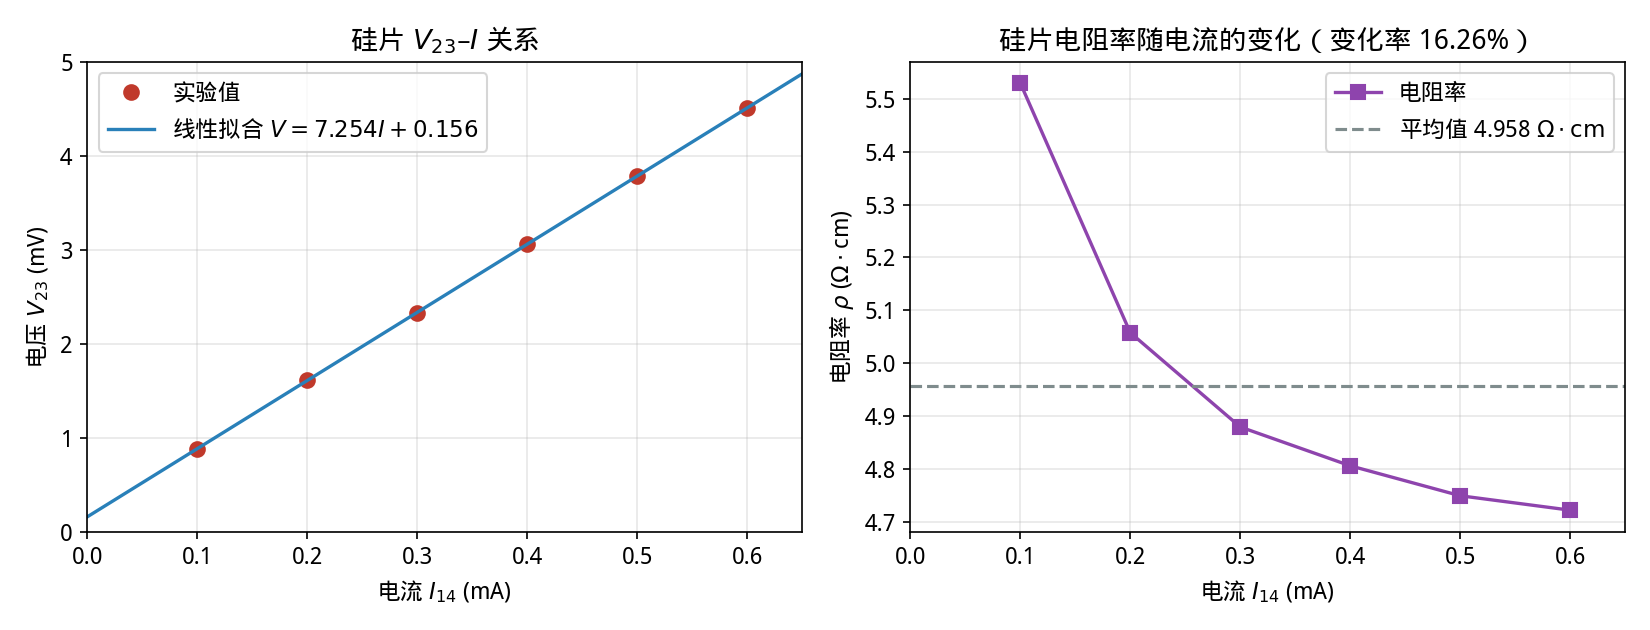
\includegraphics[width=0.92\textwidth]{images/image-2026-10-11-16-13-57.png}
\caption{硅片 $V_{23}$–$I$ 线性拟合(a)与电阻率随电流的变化(b)}
\label{fig:si}
\end{figure}

\subsection*{3. 硅片电阻率的不均匀度}
固定 $I_{14}=0.1\ \mathrm{mA}$，在样品五个区域测量，结果如下。
\begin{table}[htbp]
\centering
\caption{硅片五点电阻率（$I_{14}=0.1\ \mathrm{mA}$）}
\begin{tabular}{cccccc}
\hline
区域 & $+V_{23}$/mV & $-V_{23}$/mV & $V_{23}$/mV & $\rho$ /$\Omega\!\cdot\!$cm\\
\hline
上 & 0.92 & $-0.84$ & 0.880 & 5.529\\
中 & 0.93 & $-0.85$ & 0.890 & 5.592\\
左 & 0.91 & $-0.83$ & 0.870 & 5.466\\
右 & 0.94 & $-0.86$ & 0.900 & 5.655\\
下 & 0.92 & $-0.84$ & 0.880 & 5.529\\
\hline
\end{tabular}
\end{table}
\begin{equation}
E=\frac{5.655-5.466}{(5.655+5.466)/2}\times 100\%=3.39\%
\end{equation}

\subsection*{4. ITO 方块电阻的电流依赖性（变化率）}
\begin{table}[htbp]
\centering
\caption{ITO 方块电阻随测试电流的变化}
\begin{tabular}{ccccccc}
\hline
测点 & $I_{14}$/mA & $+V_{23}$/mV & $-V_{23}$/mV & $V_{23}$/mV & $R_{sh}$ /$\Omega\!\cdot\!\square^{-1}$\\
\hline
1 & 0.1 & 0.26 & $-0.10$ & 0.180 & 8.158\\
2 & 0.2 & 0.44 & $-0.28$ & 0.360 & 8.158\\
3 & 0.3 & 0.62 & $-0.46$ & 0.540 & 8.158\\
4 & 0.4 & 0.80 & $-0.64$ & 0.720 & 8.158\\
5 & 0.5 & 0.99 & $-0.82$ & 0.905 & 8.204\\
6 & 0.6 & 1.18 & $-1.01$ & 1.095 & 8.272\\
\hline
\end{tabular}
\end{table}
$\bar R_{sh}=8.185\ \Omega/\square$，故
\begin{equation}
C_r=\frac{8.272-8.158}{8.185}\times 100\%=1.38\%
\end{equation}
拟合得 $V_{23}=1.826\,I-0.006$（mV），$R^2=0.999884$，截距近似为零，见图 \ref{fig:ito}(a)，表明测量范围内 $R_{sh}$ 与激励电流无关，符合欧姆导电特征。

\begin{figure}[htbp]
\centering
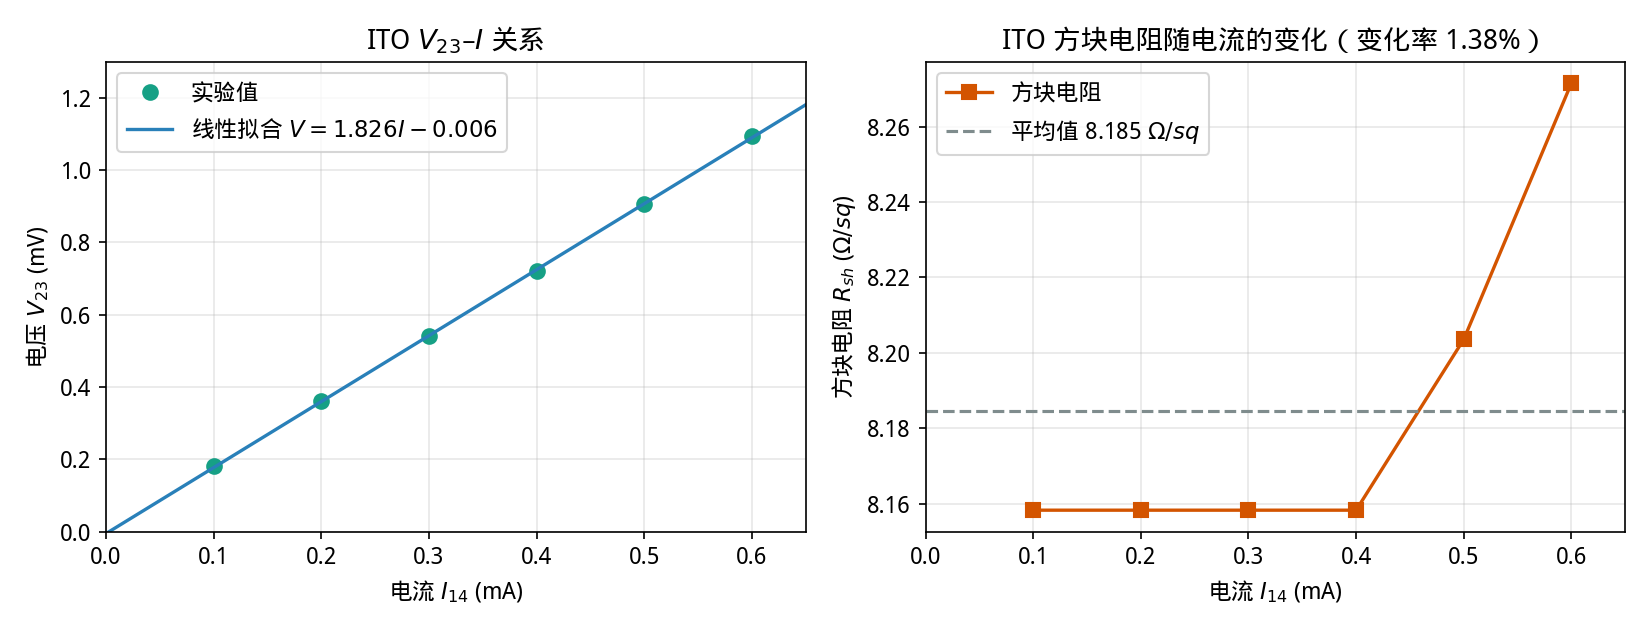
\includegraphics[width=0.92\textwidth]{images/image-2026-10-11-16-14-17.png}
\caption{ITO $V_{23}$–$I$ 线性拟合(a)与方块电阻随电流的变化(b)}
\label{fig:ito}
\end{figure}

\subsection*{5. ITO 方块电阻的不均匀度}
固定 $I_{14}=0.1\ \mathrm{mA}$，五点测试结果如下。
\begin{table}[htbp]
\centering
\caption{ITO 五点方块电阻（$I_{14}=0.1\ \mathrm{mA}$）}
\begin{tabular}{ccccc}
\hline
区域 & $+V_{23}$/mV & $-V_{23}$/mV & $V_{23}$/mV & $R_{sh}$ /$\Omega\!\cdot\!\square^{-1}$\\
\hline
上 & 0.26 & $-0.10$ & 0.180 & 8.158\\
中 & 0.27 & $-0.11$ & 0.190 & 8.612\\
左 & 0.26 & $-0.11$ & 0.185 & 8.385\\
右 & 0.27 & $-0.10$ & 0.185 & 8.385\\
下 & 0.26 & $-0.10$ & 0.180 & 8.158\\
\hline
\end{tabular}
\end{table}
\begin{equation}
E=\frac{8.612-8.158}{(8.612+8.158)/2}\times 100\%=5.41\%
\end{equation}
五点分布见图 \ref{fig:unif}。

\begin{figure}[htbp]
\centering
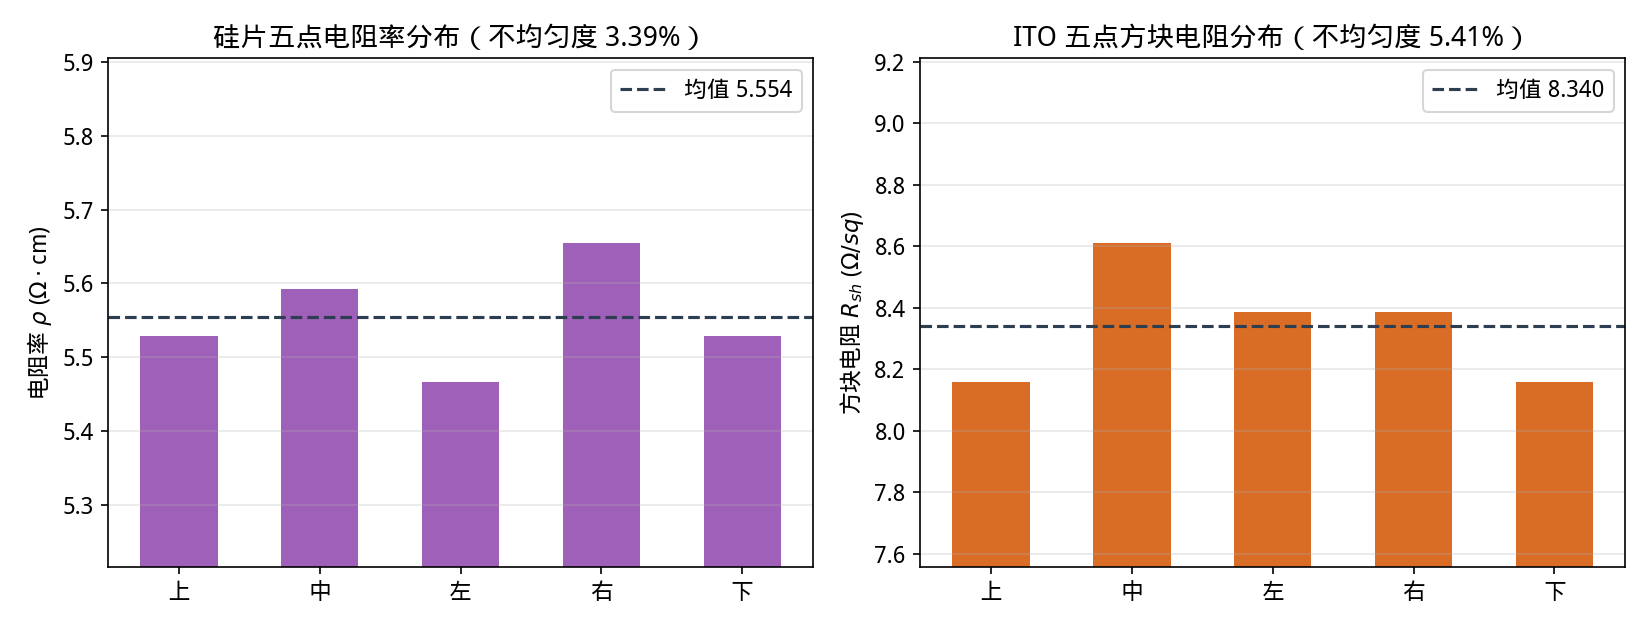
\includegraphics[width=0.92\textwidth]{images/image-2026-10-11-16-14-36.png}
\caption{硅片电阻率(a)与 ITO 方块电阻(b)的五点分布}
\label{fig:unif}
\end{figure}

\subsection*{6. 结果讨论}
\begin{enumerate}
    \item \textbf{热电势的消除。} 硅片各组满足 $(V_{+}+V_{-})/2\equiv +0.04\ \mathrm{mV}$，ITO 为 $+0.08\ \mathrm{mV}$，与电流无关且为常数，说明正反向电流平均法有效抵消了接触热电势与仪器失调，采用式（1）处理数据是必要的。
    \item \textbf{硅片变化率的成因。} $0.1\ \mathrm{mA}$ 时 $V_{23}$ 仅 $0.88\ \mathrm{mV}$，源表分辨率与噪声的相对贡献显著，读数偏高；随电流增大信噪比改善，$\rho$ 趋于 $4.72\ \Omega\!\cdot\!\mathrm{cm}$ 的饱和值。同时大电流下的焦耳热使晶格温度升高、载流子迁移率下降，并可能伴有非平衡载流子注入，均使测得电阻率略低于小电流值。故材料本征电阻率宜取饱和区的 $4.72\ \Omega\!\cdot\!\mathrm{cm}$。
    \item \textbf{ITO 的稳定性。} $R_{sh}$ 变化率仅 $1.38\%$，$V$–$I$ 拟合截距近似为零，表明 ITO 薄膜与探针形成良好欧姆接触，$0.1\sim0.6\ \mathrm{mA}$ 范围内无明显自热与非线性效应，方块电阻测得值可信度高。
    \item \textbf{面内均匀性。} 硅片不均匀度 $3.39\%$，反映单晶拉制与掺杂的面内一致性较好；ITO 不均匀度 $5.41\%$，略高于硅片。由于 $R_{sh}=\rho/d$，方阻对膜厚波动极为敏感，溅射成膜时膜厚与氧空位浓度的面内起伏被直接放大为方阻起伏，这与薄膜工艺的本征离散性一致。
    \item \textbf{修正系数的适用性。} 硅片厚度 $d=0.2\ \mathrm{mm}=0.2S$，不满足 $d>4S$ 的半无穷大条件，严格计算应引入厚度修正系数 $B_0$。本实验按式（2）直接计算，所得为表观电阻率；若需精确值，应根据 $d/S=0.2$ 查表取 $B_0$ 并由 $\rho=2\pi S B_0^{-1}(V_{23}/I)$ 修正。ITO 满足 $d\ll S$，可直接使用式（3），无需修正。
\end{enumerate}

\section*{实验结论（20分）}
\begin{enumerate}
    \item \textbf{测量方法的有效性得到验证。} 硅片与 ITO 的 $V_{23}$–$I$ 关系均呈高度线性（$R^2$ 分别为 $0.999996$ 与 $0.999884$），且正反向电流读数之和恒为常数（硅片 $+0.04\ \mathrm{mV}$，ITO $+0.08\ \mathrm{mV}$），证明四线法接线消除了引线电阻与接触电阻的影响，正反电流平均法有效抵消了寄生热电势，实验数据可靠。

    \item \textbf{硅片电阻率。} 在 $0.1\sim0.6\ \mathrm{mA}$ 范围内，测得电阻率由 $5.53\ \Omega\!\cdot\!\mathrm{cm}$ 单调下降并趋于饱和值 $4.72\ \Omega\!\cdot\!\mathrm{cm}$，$\bar\rho=4.96\ \Omega\!\cdot\!\mathrm{cm}$，变化率 $C_r=16.26\%$。该变化率并非材料本征性质，而是小电流下信噪比不足与大电流下焦耳热效应共同作用的结果，材料本征电阻率应取饱和区数值 $4.72\ \Omega\!\cdot\!\mathrm{cm}$。五点测试得 $\rho_{\max}=5.655$、$\rho_{\min}=5.466\ \Omega\!\cdot\!\mathrm{cm}$，不均匀度 $E=3.39\%$，表明单晶硅片掺杂面内一致性良好。

    \item \textbf{ITO 方块电阻。} 方块电阻在 $8.16\sim8.27\ \Omega/\square$ 之间，$\bar R_{sh}=8.18\ \Omega/\square$，变化率仅 $1.38\%$，拟合截距近似为零，说明 ITO 薄膜与探针形成良好欧姆接触，测试电流范围内无自热与非线性效应，方阻测量可信度高，且方阻与激励电流无关，符合欧姆导电规律。五点测试得 $R_{sh,\max}=8.612$、$R_{sh,\min}=8.158\ \Omega/\square$，不均匀度 $E=5.41\%$。

    \item \textbf{两类样品的对比。} ITO 的电学稳定性（变化率 $1.38\%$）显著优于硅片（$16.26\%$），而其面内均匀性（不均匀度 $5.41\%$）略逊于硅片（$3.39\%$）。原因在于 $R_{sh}=\rho/d$，方阻对膜厚极其敏感，薄膜沉积的膜厚与氧空位面内起伏被直接放大为方阻起伏；而硅片为体单晶，掺杂由拉晶工艺决定，面内一致性更好。

    \item \textbf{修正系数的适用性。} 硅片厚度 $d=0.2\ \mathrm{mm}=0.2S$，不满足半无穷大条件 $d>4S$，本实验所得为表观电阻率，严格值需引入厚度修正系数 $B_0$；ITO 满足 $d\ll S$，可直接使用极薄样品公式，无需修正。双电测组合四探针法因结果与探针间距无关、可自动修正边界效应，在薄层电阻精密测量中优于经典直排法。
\end{enumerate}

\section*{实验启示和拓展（10分）}
\begin{enumerate}
    \item \textbf{激励条件的选择。} 本实验表明注入电流并非越大越好：电流过小则信噪比不足，过大则引起焦耳热与非平衡载流子注入。实际测试中应在 $V$–$I$ 线性区选取中等偏大的电流，并以正反向平均消除失调，这是电学表征中平衡精度与扰动的基本策略。

    \item \textbf{由电阻率到掺杂浓度。} 测得 $\rho$ 后，由 $\rho=1/(q\mu_p N_A)$（p 型）或 $\rho=1/(q\mu_n N_D)$（n 型）可反推掺杂浓度。关键在于迁移率 $\mu$ 本身依赖于载流子浓度，需采用 Caughey--Thomas 等经验迁移率模型迭代求解，或查阅 ASTM F723 标准 $\rho$–$N$ 换算曲线；对补偿半导体还需考虑离化率与温度修正，必要时应以霍尔测试独立测定载流子浓度与迁移率以分离两者贡献。

    \item \textbf{ITO 方阻对器件性能的影响。} 方阻直接决定透明电极的串联电阻与横向压降：方阻过大将导致 OLED、太阳能电池等器件的电流分布不均、发光或取光效率下降、局部发热与填充因子劣化；方阻过小则需增厚膜层，而 ITO 在可见光短波与近红外区存在自由载流子吸收，膜厚增加必然牺牲透光率。因此方阻设计本质是导电性与透光率的折中，工程上常以品质因数 $\Phi_{\mathrm{TC}}=T^{10}/R_{sh}$ 综合评价；同时方阻的面内不均匀会直接转化为器件亮度或响应的不均匀，是量产良率的关键控制指标。

    \item \textbf{测量方法的拓展。} 针对微小图形区、超浅结与高方阻样品，可进一步采用范德堡法、扩展电阻探针（SRP）与霍尔效应测试；对薄层结构的纵向载流子分布，则需借助四探针配以逐层剥离或斜角磨角技术获得扩展电阻深度剖面。此外，将四探针法与温控平台结合，可由电阻率的温度依赖性提取杂质电离能，实现掺杂类型的辅助判别。
\end{enumerate}


\end{document}